\documentclass[11pt]{article}
\usepackage[a4paper,margin=24mm]{geometry}
\usepackage{amsmath,amssymb,microtype,pgfplots}
\pgfplotsset{compat=1.18}
\title{Vortex shedding behind a circular cylinder at low Reynolds number}
\author{A.~Author \and B.~Author}
\date{}
\begin{document}
\maketitle
\begin{abstract}
We revisit the onset of periodic vortex shedding in the wake of a circular cylinder.
A global linear stability analysis of the steady base flow predicts the critical
Reynolds number $\mathrm{Re}_c \approx 46.7$ and the Strouhal number of the emerging
limit cycle within one per cent of direct numerical simulation.
\end{abstract}

\section{Introduction}
The wake of a bluff body is the canonical example of a globally unstable flow.
Above a critical Reynolds number the steady, symmetric recirculation bubble gives way
to the periodic von K\'arm\'an street, whose frequency is set by a self-excited
global mode rather than by the upstream forcing.

\section{Governing equations}
The incompressible flow $\mathbf{u}(\mathbf{x},t)$ obeys
\begin{equation}
\partial_t \mathbf{u} + (\mathbf{u}\cdot\nabla)\mathbf{u} = -\nabla p + \frac{1}{\mathrm{Re}}\,\Delta\mathbf{u},
\qquad \nabla\cdot\mathbf{u} = 0 .
\label{eq:ns}
\end{equation}
Linearising \eqref{eq:ns} about the steady base flow $\mathbf{U}$ and seeking
$\mathbf{u}' = \hat{\mathbf{u}}\,e^{\lambda t}$ gives the eigenvalue problem
\begin{equation}
\lambda\,\hat{\mathbf{u}} = -(\mathbf{U}\cdot\nabla)\hat{\mathbf{u}} - (\hat{\mathbf{u}}\cdot\nabla)\mathbf{U}
- \nabla\hat p + \frac{1}{\mathrm{Re}}\,\Delta\hat{\mathbf{u}} .
\end{equation}

\section{Results}
The growth rate $\sigma = \Re(\lambda)$ of the leading mode crosses zero at
$\mathrm{Re}_c = 46.7$ (figure~\ref{fig:growth}).

\begin{figure}[h]
\centering
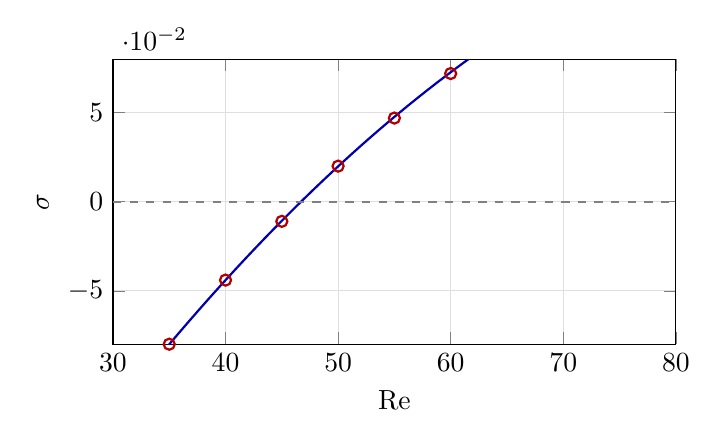
\begin{tikzpicture}
\begin{axis}[width=0.72\textwidth,height=5.2cm,xlabel={$\mathrm{Re}$},ylabel={$\sigma$},
  grid=major,grid style={gray!25},xmin=30,xmax=80,ymin=-0.08,ymax=0.08,
  every axis plot/.append style={thick}]
\addplot[blue!70!black,domain=30:80,samples=60] {0.0062*(x-46.7)-0.000055*(x-46.7)^2};
\addplot[only marks,mark=o,red!70!black] coordinates {(35,-0.08)(40,-0.044)(45,-0.011)(50,0.020)(55,0.047)(60,0.072)};
\addplot[dashed,gray] coordinates {(30,0)(80,0)};
\end{axis}
\end{tikzpicture}
\caption{Growth rate of the leading global mode against Reynolds number:
linear stability (line) and direct numerical simulation (circles).}
\label{fig:growth}
\end{figure}

The Strouhal number at onset, $\mathrm{St} = 0.118$, matches the frequency of the
saturated limit cycle within one per cent.
\end{document}
